\documentclass[submit]{harvardml}

\course{CS181-S21}
\assignment{Assignment \#3}
\duedate{7:59pm EST, March 5, 2021}

\usepackage[OT1]{fontenc}
\usepackage[colorlinks,citecolor=blue,urlcolor=blue]{hyperref}
\usepackage[pdftex]{graphicx}
\usepackage{subfig}
\usepackage{fullpage}
\usepackage{amsmath}
\usepackage{amssymb}
\usepackage{color}
\usepackage{soul}
\usepackage{todonotes}
\usepackage{listings}
\usepackage{common}
\usepackage{enumitem}
\usepackage{bm}
\usepackage{listings}
\usepackage{physics}
\usepackage[shortlabels]{enumitem}
\newcommand{\B}{\text{B}}
\newcommand{\Beta}{\text{Beta}}

\usepackage[mmddyyyy,hhmmss]{datetime}

\definecolor{verbgray}{gray}{0.9}

\lstnewenvironment{csv}{%
  \lstset{backgroundcolor=\color{verbgray},
  frame=single,
  framerule=0pt,
  basicstyle=\ttfamily,
  columns=fullflexible}}{}

\begin{document}

\begin{center}
{\Large Homework 3: Bayesian Methods and Neural Networks}\\
\end{center}

\subsection*{Introduction}

This homework is about Bayesian methods and Neural Networks.  Section 2.9 in the textbook as well as reviewing MLE and MAP will be useful for Q1. Chapter 4 in the textbook will be useful for Q2.

Please type your solutions after the corresponding problems using this
\LaTeX\ template, and start each problem on a new page.

Please submit the \textbf{writeup PDF to the Gradescope assignment `HW3'}. Remember to assign pages for each question.  \textbf{All plots you submit must be included in your writeup PDF.  }We will not be checking your code / source files except in special circumstances. 

Please submit your \textbf{\LaTeX file and code files to the Gradescope assignment `HW3 - Supplemental'}. 


\begin{problem}[Bayesian Methods]

  This question helps to build your understanding of making
  predictions with a maximum-likelihood estimation (MLE), a maximum a
  posterior estimator (MAP), and a full posterior predictive.

  Consider a scalar variable $x$ with the following generative
  process: First, the mean $\mu$ is sampled from a prior
  $N(0,\tau^2)$.  Next, each $x_n$ is generated as $x_n = \mu +
  \epsilon_n$, where $\epsilon_n \sim N(0,\sigma^2)$. All
  $\epsilon_n$'s are independent of each other and of $\mu$.

  For this problem, use $\sigma^2 = 1$ and $\tau^2 = 5$.  

  Now, we see 14 independent samples of $x$ to yield data
  $$D = 3.3, 3.5, 3.1, 1.8, 3.0, 0.74, 2.5, 2.4, 1.6, 2.1, 2.4, 1.3, 1.7, 0.19$$
    
  \textit{Make sure to include all required plots in your PDF.}

\begin{enumerate}

\item Derive the expression for $p(\mu|D)$.  Do \emph{not} plug in
  numbers yet!

  Hint: Use properties of normal-normal conjugacy to simplify your derivation.  You can also refer to \href{https://www.cs.ubc.ca/~murphyk/Papers/bayesGauss.pdf}{this paper}.
  
\item Now we get to our core interest: the predictive distribution of
  a new datapoint $x^*$ given our observed data $D$, $p(x^*|D)$.
  Write down the expression for the full posterior predictive
  distribution: $$p(x^*|D) = \int p(x^*|\mu)p(\mu|D) d\mu$$ Interpret
  your expression in a few words.  Do \emph{not} plug in numbers yet!

  Hint: To simplify your derivation,
  use the fact that $x = \mu + \epsilon$, and $\mu|D$ and $\epsilon$
  are independent Gaussians whose distributions you know from above.
  
\item The full posterior predictive distribution had a nice analytic
  form in this case, but in many problems, it is often difficult to
  calculate because we need to marginalize out the parameters (here,
  the parameter is $\mu$). We can mitigate this problem by plugging in
  a point estimate of $\mu^*$ rather than a distribution. Derive the
  estimates of $p(x^*|D) \approx p(x^*|\mu^*)$ for $\mu^* = \mu_{MLE}$
  and $\mu^* = \mu_{MAP}$.  How do these expressions compare to the
  expression for the full posterior above? Do \emph{not} plug in
  numbers yet!
  
   
\item Plot how the above 3 distributions change after each data point
  is gathered.  You will have a total of 15 plots, starting with the
  plot for the case with no data (they can be small, e.g. in a $3\times5$
  grid).  The x-axis of each plot will be the $x$ value and the y-axis
  the density.  You can make one plot for each estimator, or combine
  all three estimators onto one plot with a different colored line for
  each estimator.
  
    
\item How do the means of the predictive distributions vary with more
  data?  How do the variances vary?  Interpret the differences you see
  between the three different estimators.
  
  \item Does the ordering of the data matter for the final predictive
  distributions?  

  \item Derive an expression for and then compute the marginal
    likelihood of the training data $p(D)$.

    Hint: You can rearrange the required integral such that it looks like an un-normalized
    Gaussian distribution in terms of $\mu$,  and take advantage of the fact that
    integrating over a normalized Gaussian distribution is equal to 1.
    You will need to complete the square.
    
  \item Now consider an alternate model in which we were much more sure
  about the mean: $\mu \sim N(0,\tau^2)$, where $\tau^2 = 0.1$.
  Compute the marginal likelihood $p(D)$ for this model.  Which of the
  two models has a higher marginal likelihood? Interpret this result.

\end{enumerate}

\end{problem}

\subsection*{Solution:}

\begin{enumerate}
    \item Using the results of the paper, as well as Normal-Normal conjugacy, we see that $\mu|D$ is normally distributed with mean $\frac{\sum_i x_i}{\sigma^2(\frac{n}{\sigma^2} + \frac{1}{\tau^2})}$ and variance $\frac{1}{\frac{n}{\sigma^2} + \frac{1}{\tau^2}}$. Therefore, we see that 
    
    $$p(\mu|D) = \frac{1}{\sqrt{2\pi \frac{1}{\frac{n}{\sigma^2} + \frac{1}{\tau^2}}}}\exp{-\frac{\frac{n}{\sigma^2} + \frac{1}{\tau^2}}{2}(\mu - \frac{\sum_i x_i}{\sigma^2(\frac{n}{\sigma^2} + \frac{1}{\tau^2})})^2}$$
    
    \item $p(x^*|D) = \int p(x^*|\mu)p(\mu|D) d\mu = \int N(x|\mu, \sigma) N(\mu|\mu_n, \sigma_n^2)d\mu$, where $\mu_n = \frac{\sum_i x_i}{\sigma^2(\frac{n}{\sigma^2} + \frac{1}{\tau^2})}$ and $\sigma_n^2 = \frac{1}{\frac{n}{\sigma^2} + \frac{1}{\tau^2}}$ from above. From general properties of the Gaussian distribution, this means that $p(x^*|D) = N(\frac{\sum_i x_i}{\sigma^2(\frac{n}{\sigma^2} + \frac{1}{\tau^2})}, \sigma^2 + \frac{1}{\frac{n}{\sigma^2} + \frac{1}{\tau^2}})$.
    
    
    The variance in this expression captures the uncertainty due to the observation noise plus the uncertainty due to the parameters. The mean is updated in a way such that over time and with more data, $n$ comes to dominate the denominator, pushing the mean of the distribution toward the sample mean.
    
    \item For $\mu_{\text{MLE}}$, we want to find the $\mu^*$ that maximizes the log likelihood of $\mu|D$. We see the following:
    
    $L = \log(p(\mu|D)) = \log(\prod_{x\in D} p(x)) = \log(\prod_{x\in D} p(\epsilon = x - \mu)) = \sum_{x\in D} \log(\frac{1}{\sqrt{2\pi\sigma^2}}\exp{-\frac{1}{2}(\frac{x-\mu}{\sigma})^2})$.
    
    We want to find the $\mu_{\text{MLE}}$ that maximizes this so we take its derivative with respect to $\mu$. This gives us :
    
    $$\pdv{L}{\mu} = \frac{1}{2}\sum_{x \in D} (\frac{x-\mu}{\sigma})^2 = 0$$
    
    $$\sum_{x \in D} \mu = \sum_{x \in D} x$$
    
    $$\mu = \mu_{\text{MLE}} = \frac{\sum_{x \in D}}{|D|}$$
    
    This means that $p(x^*|\mu_{\text{MLE}}) = \frac{1}{\sqrt{2\pi \sigma^2}} \exp{-\frac{1}{2}(\frac{x^* - \mu_{\text{MLE}}}{\sigma})^2}$
    
    For $\mu_{\text{MAP}}$, we want to find the mode of the distribution of $\mu|D$ found previously. We know that $p(\mu|D)$ is proportinoal to $p(D|\mu)p(\mu)$. We see the following:
    
    $p(\mu|D)  = [\prod_{x \in D} p(\epsilon = x-\mu)]p(\mu)$.
    
    We can take a log of this expression and the $\mu$ that maximizes the logged expression will still maximize our original expression, but calculations will be easier. We want to find the $\mu$ then that maximizes the following:
    
    $\sum_{x \in D} [\log p(\epsilon = x - \mu)] + \log p(\mu)$.
    
    Rewriting this and removing unnecessary terms that don't depend on $\mu$, we see that we will take the derivative of the following expression with respect to $\mu$ and set it to 0 to get our $\mu_{\text{MAP}}$:
    
    $$\sum_{x \in D} [\frac{1}{2}(\frac{x-\mu}{\sigma^2})^2] + \frac{1}{2}(\frac{\mu}{\tau})^2$$.
    
    Taking the derivative we get:
    
    $$-\frac{1}{\sigma^2}\sum_{x \in D} (x-\mu) + \frac{\mu}{\tau^2} = 0$$
    
    $$-\frac{1}{\sigma^2} \sum_{x \in D} + \frac{n\mu}{\sigma^2} + \frac{\mu}{\tau^2} = 0$$
    
    $$\mu_{\text{MAP}} = \frac{\sum_{x \in D}x}{\frac{\sigma^2}{\tau^2}+n}$$
    
    This means that $p(x^*|\mu_{\text{MAP}}) = \frac{1}{\sqrt{2\pi \sigma^2}} \exp{-\frac{1}{2}(\frac{x^* - \mu_{\text{MAP}}}{\sigma})^2}$
    
    The MAP-approximator, like the posterior predictive, considers the prior distribution in the mean of its associated predictive distribution. However, both the MLE-approximate and the MAP-approximate maintain the prior variance. The MLE-approximator's mean entire relies on the sample data. However, with enough data, all these approximators' means should converge to a similar value. 
    
    \item Plots:
    
    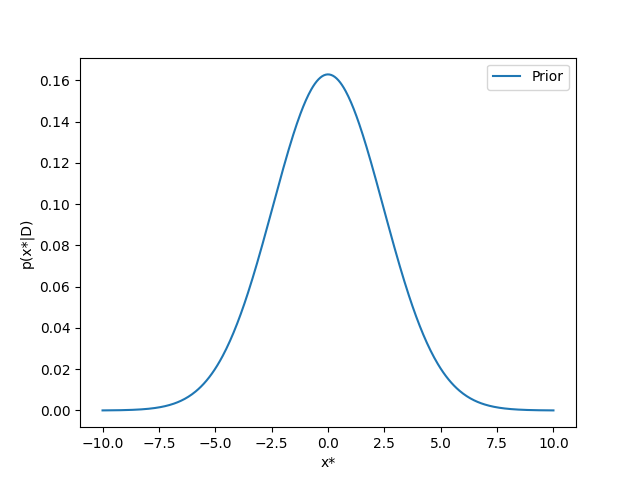
\includegraphics[width=.3\textwidth]{base.png}
    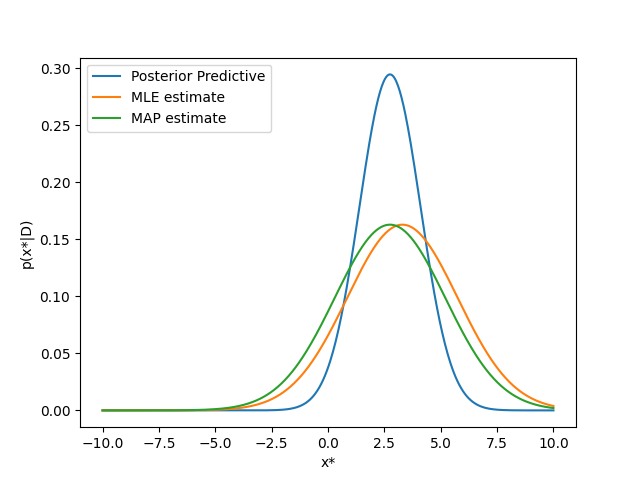
\includegraphics[width=.3\textwidth]{iter1.png}
    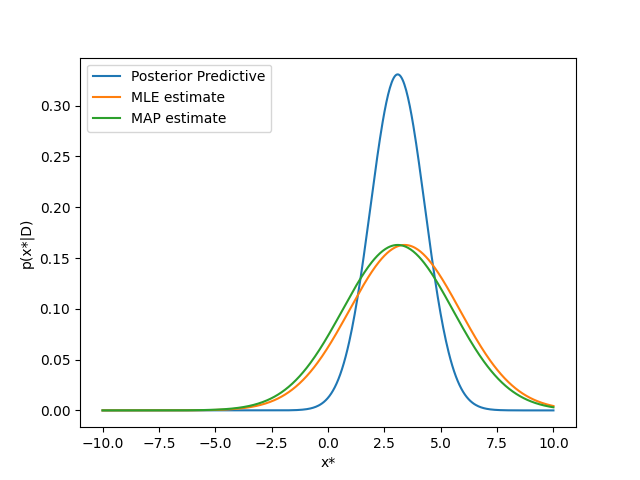
\includegraphics[width=.3\textwidth]{iter2.png}
    
    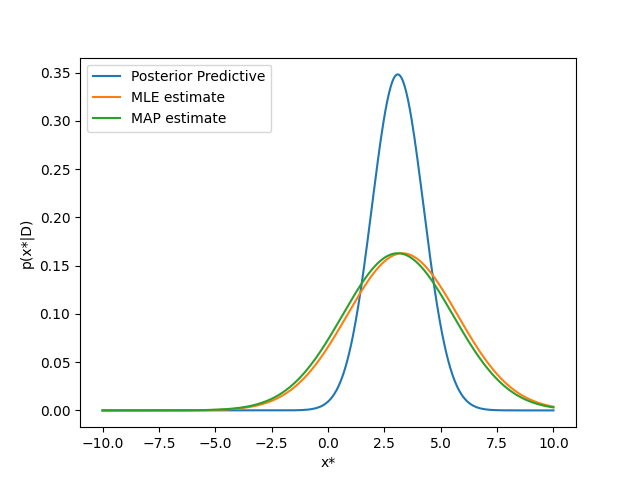
\includegraphics[width=.3\textwidth]{iter3.png}
    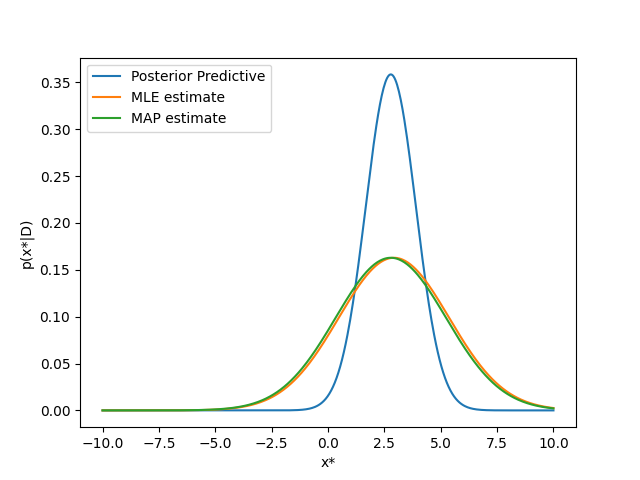
\includegraphics[width=.3\textwidth]{iter4.png}
    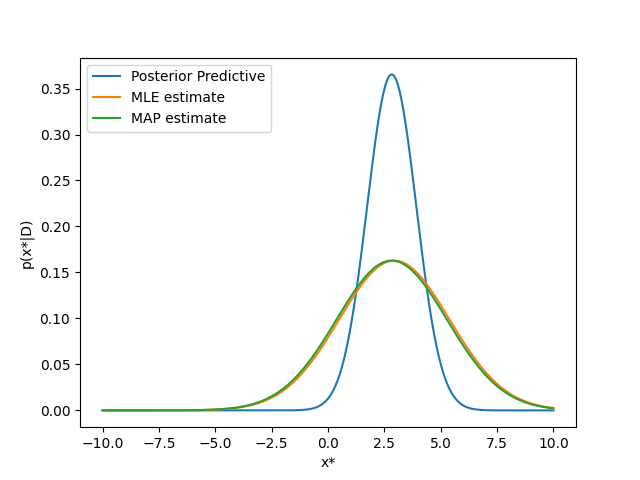
\includegraphics[width=.3\textwidth]{iter5.png}
    
    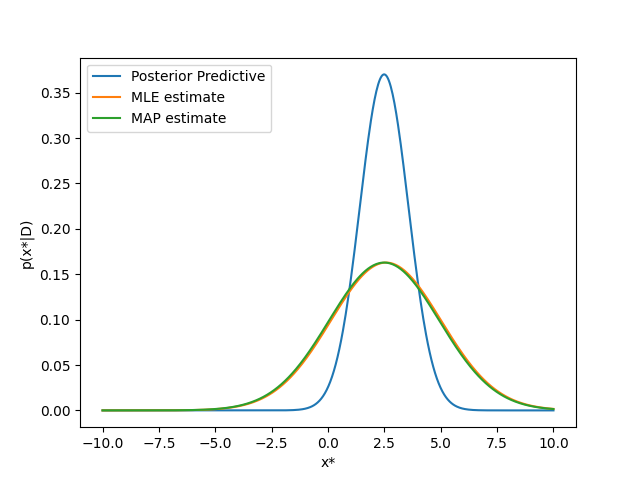
\includegraphics[width=.3\textwidth]{iter6.png}
    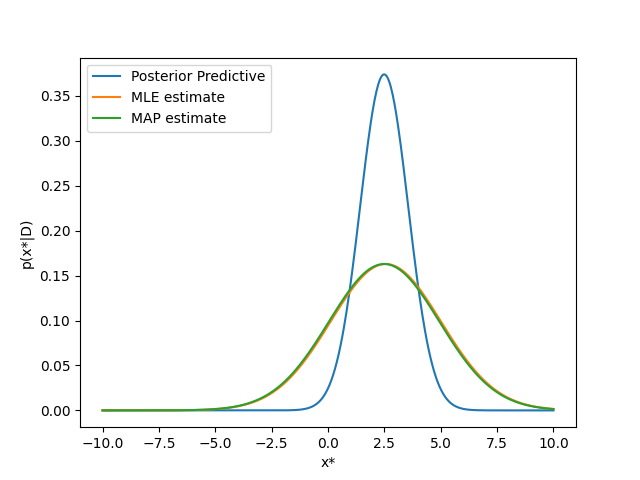
\includegraphics[width=.3\textwidth]{iter7.png}
    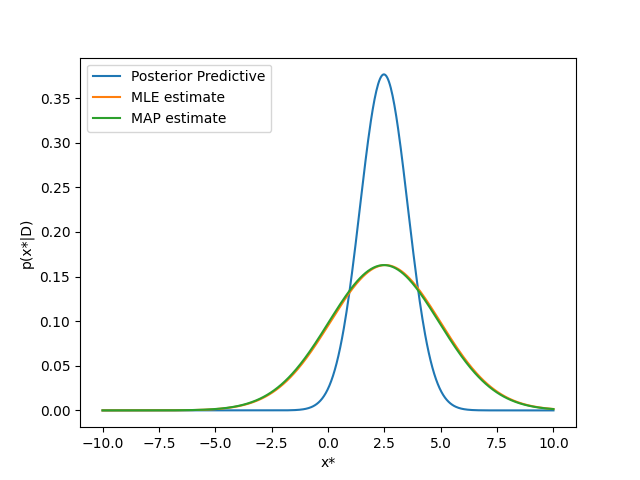
\includegraphics[width=.3\textwidth]{iter8.png}
    
    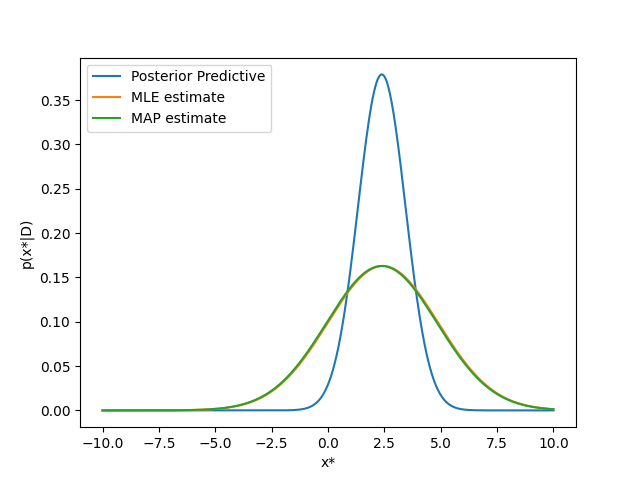
\includegraphics[width=.3\textwidth]{iter9.png}
    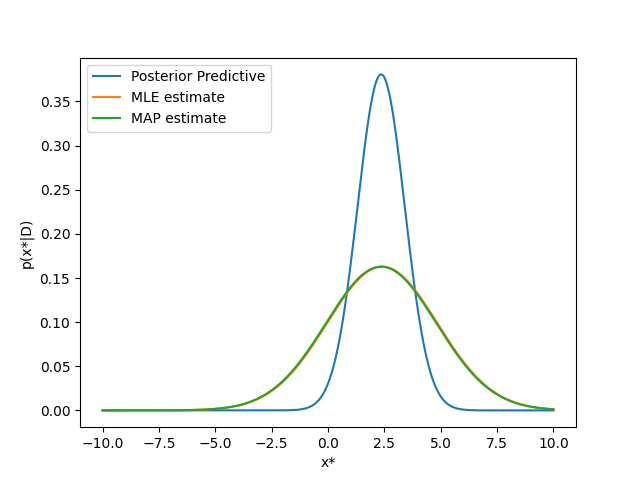
\includegraphics[width=.3\textwidth]{iter10.png}
    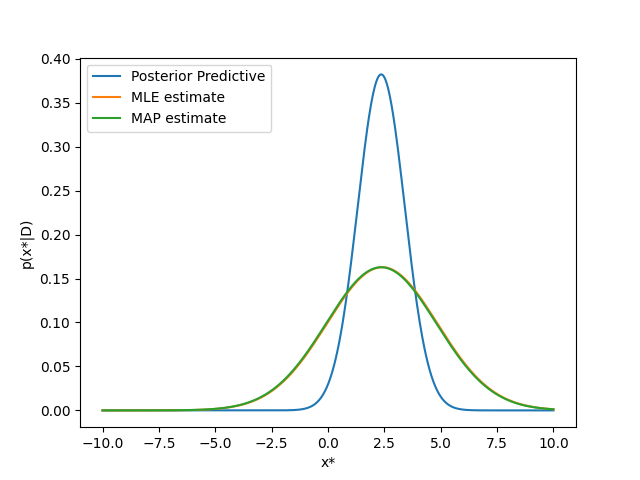
\includegraphics[width=.3\textwidth]{iter11.png}
    
    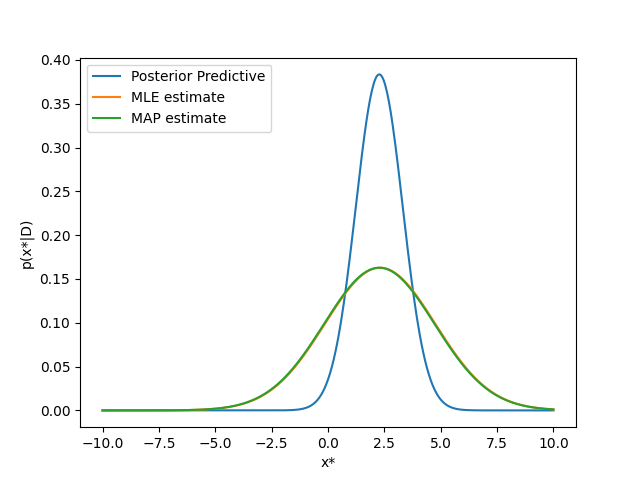
\includegraphics[width=.3\textwidth]{iter12.png}
    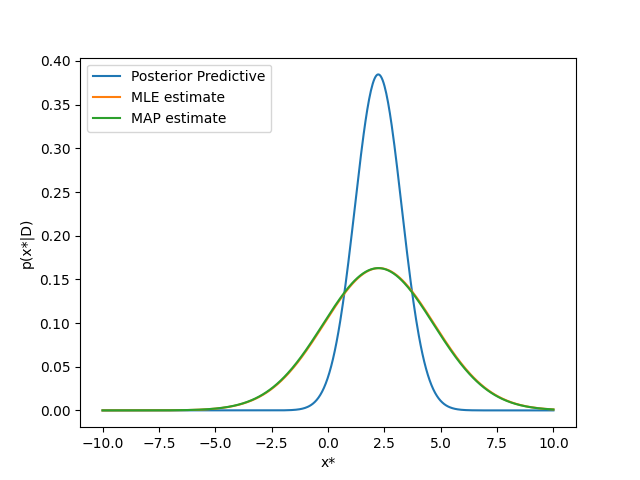
\includegraphics[width=.3\textwidth]{iter13.png}
    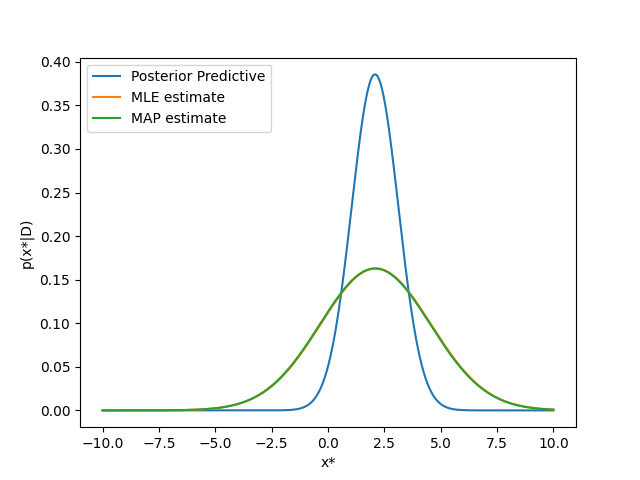
\includegraphics[width=.3\textwidth]{iter14.png}
    
    \item The means of the posterior predictive distribution and the MAP-estimated posterior get closer to the sample mean of the data as we get more data. The mean of the MLE-estimated poterior is always exactly the sample mean. The variances of the MAP-estimated and the MLE-estimated predictive distributions will remain at the variance of the prior distribution, while the variance of the posterior predictive will decrease. We can see this mathematically for the posterior predictive since as $n$ increases, the variance of the posterior predictive distribution will decrease. Then, since the mean of the posterior predictive can be written in terms of its variance, as variance decreases and becomes dominated by the $n$ term, similarly, the effect of other terms in the expression for the mean will become less important/cancel out, leaving the sample mean to prevail. The MAP-estimated predictive is affected by both the sample data and the prior, but similarly, as we get more data, its mean will tend toward the sample mean. Eventually, the effect of our real observations will shift us away from our assumed prior and toward the distribution encouraged by observations, which should be indicative, with a large enough dataset, of the true distribution.
    
    \item The ordering of the data does not matter for the final predictive distributions. We can see for the posterior predictive that variance updates dependent on the previous variance, but this is order agnostic. Similarly, the mean updates with the average of data observed so far, but order doesn't matter since it depends only on prior variance and updated variance, both of which are order agnostic. For the MLE-approximation, the mean is always the sample mean, and for the MAP-approximation, the mean depends on the sample mean and the variance, which stays constant at the variance of the prior (same for MLE-approximation). 
    
    \item 
    
    $p(D) = \int_{-\infty}^{\infty} p(D|\mu)p(\mu) d\mu = \int [\prod_{i=1}^n N(x_i | \mu, \sigma^2)]N(0, \tau^2)d\mu = \int[\prod_{i=1}^n \frac{1}{\sigma\sqrt{2\pi}}\exp{-\frac{1}{2}(\frac{x_i-\mu}{\sigma})^2}] \frac{1}{\tau\sqrt{2\pi}} \exp{-\frac{1}{2}(\frac{\mu}{\tau})^2}d\mu$
    
    $= \frac{1}{(\sigma\sqrt{2\pi})^n(\tau\sqrt{2\pi})}\int \exp(-\frac{1}{2\sigma^2}\sum_{i=1}^n (x_i - \mu)^2 - \frac{1}{2\tau^2}\mu^2)d\mu$
    
    Within in the integral of the expression, we see that:
    
    $\exp(-\frac{1}{2\sigma^2}\sum_{i=1}^n (x_i - \mu)^2 - \frac{1}{2\tau^2}\mu^2)d\mu $
    
    $\exp(-\frac{1}{2\sigma^2}(\sum{i=1}^n x_i^2) - \frac{1}{2\sigma^2}n\mu^2 - \frac{1}{2\tau^2}\mu^2 + \frac{\mu}{\sigma^2}\sum{i=1}^n x_i)$
    
    Moving constants outside the integral, we rewrite the full expression as:
    
    $\frac{\exp(-\frac{1}{2\sigma^2}\sum_{i=1}^n x_i^2)}{(\sigma\sqrt{2\pi})^n(\tau\sqrt{2\pi})}\int \exp(-\frac{1}{2}(\frac{1}{\sigma^2}n + \frac{1}{\tau^2})(\mu^2 - 2\mu\frac{\frac{1}{\sigma^2}\sum_{i=1}^n x_i}{\frac{n}{\sigma^2} + \frac{1}{\tau^2}})) d\mu$
    
    By completing the square by adding the requisite constant terms and moving things outside the integral where possible, we get:
    
    $\frac{\exp(-\frac{1}{2\sigma^2}\sum_{i=1}^n x_i^2)}{(\sigma\sqrt{2\pi})^n(\tau\sqrt{2\pi})}\exp(\frac{(\frac{1}{\sigma^2}\sum_{i=1}^n x_i)^2}{2(\frac{n}{\sigma^2} + \frac{1}{\tau^2})}) \int \frac{\sqrt{2\pi}}{\sqrt{2\pi}} \exp(-\frac{1}{2}(\frac{1}{\sigma^2}n + \frac{1}{\tau^2})(\mu - \frac{\frac{1}{\sigma^2}\sum_{i=1}^n x_i}{\frac{n}{\sigma^2} + \frac{1}{\tau^2}})^2) d\mu$
    
    The integral integrates to $\frac{\sqrt{2\pi}}{\sqrt{\frac{n}{\sigma^2} + \frac{1}{\tau^2}}}$, so we can rewrite the full expression as:
    
    $p(D) = \frac{\exp(-\frac{1}{2\sigma^2}\sum_{i=1}^n x_i^2)}{(\sigma\sqrt{2\pi})^n(\tau\sqrt{2\pi})}\exp(\frac{(\frac{1}{\sigma^2}\sum_{i=1}^n x_i)^2}{2(\frac{n}{\sigma^2} + \frac{1}{\tau^2})})\frac{\sqrt{2\pi}}{\sqrt{\frac{n}{\sigma^2} + \frac{1}{\tau^2}}}$
    
    Substituting in values, we get:
    
    $p(D) = \frac{\exp(-\frac{1}{2}(74.8937))}{(\sqrt{2\pi})^{14}(\sqrt{10\pi})}\exp(\frac{(29.63)^2}{2(14 + \frac{1}{5})})\frac{\sqrt{2\pi}}{\sqrt{2(14 + \frac{1}{5})}} = 3.15573*10^{-10}$
    
    \item 
    
    Substituting in values, we get:
    
    $p(D) = \frac{\exp(-\frac{1}{2}(74.8937))}{(\sqrt{2\pi})^{14}(\sqrt{0.2\pi})}\exp(\frac{(29.63)^2}{2(14 + 10)})\frac{\sqrt{2\pi}}{\sqrt{2(14 + 10)}} = 5.65665*10^{-15}$
    
    The original model had the higher marginal likelihood because the sample data has mean that is sufficiently far from zero that if we think we are more certain the true mean is 0, then it's less likely that we would have seen the data we have in these 14 samples, which have a mean skewed well in to positive.
    
\end{enumerate}

\newpage
\begin{problem}[Neural Net Optimization]

  In this problem, we will take a closer look at how gradients are calculated for backprop with a simple multi-layer perceptron (MLP). The MLP will consist of a first fully connected layer with a sigmoid activation, followed by a one-dimensional, second fully connected layer with a sigmoid activation to get a prediction for a binary classification problem. Assume bias has not been merged. Let:
  \begin{itemize}
      \item $\bold{W}_1$ be the weights of the first layer, $\bold{b}_1$ be the bias of the first layer.
      \item $\bold{W}_2$ be the weights of the second layer, $\bold{b}_2$ be the bias of the second layer.
  \end{itemize}
  
  The described architecture can be written mathematically as: $$\hat{y} = \sigma(\bold{W}_2 \left[\sigma \left(\bold{W}_1 \bold{x} + \bold{b}_1\right)\right] + \bold{b}_2)$$
  
  where $\hat{y}$ is a scalar output of the net when passing in the single datapoint $\bold{x}$ (represented as a column vector), the additions are element-wise additions, and the sigmoid is an element-wise sigmoid.
  
  \begin{enumerate}
      \item Let:
      \begin{itemize}
          \item $N$ be the number of datapoints we have
          \item $M$ be the dimensionality of the data
          \item $H$ be the size of the hidden dimension of the first layer. Here, hidden dimension is used to describe the dimension of the resulting value after going through the layer. Based on the problem description, the hidden dimension of the second layer is 1.
      \end{itemize}
      
      Write out the dimensionality of each of the parameters, and of the intermediate variables:

          \begin{align*}
          \bold{a}_1 &= \bold{W}_1 \bold{x} + \bold{b}_1, 
          &\bold{z}_1 = \sigma(\bold{a}_1) \\
          a_2 &= \bold{W}_2 \bold{z}_1 + \bold{b}_2, 
          &\hat{y} = z_2 = \sigma(a_2)
          \end{align*}
          
      and make sure they work with the mathematical operations described above.
      
    \item  We will derive the gradients for each of the parameters.  The gradients can be used in gradient descent to find weights that improve our model's performance. For this question, assume there is only one datapoint $\bold{x}$, and that our loss is $L = -(y \log (\hat{y}) + (1 - y) \log (1 - \hat{y}))$. For all questions, the chain rule will be useful.
    \begin{enumerate}
        \item Find $\frac{\partial L}{\partial b_2}$. 
        
        \item Find $\frac{\partial L}{\partial W_2^h}$, where $W_2^h$ represents the $h$th element of $\bold{W}_2$.
        
        \item Find $\frac{\partial L}{\partial b_1^h}$, where $b_1^h$ represents the $h$th element of $\bold{b}_1$. (*Hint: Note that only the $h$th element of $\bold{a}_1$ and $\bold{z}_1$ depend on $b_1^h$ - this should help you with how to use the chain rule.)
        
        \item Find $\frac{\partial L}{\partial W_1^{h,m}}$, where  $W_1^{h,m}$ represents the element in row $h$, column $m$ in $\bold{W}_1$.
    
    \end{enumerate}
    \end{enumerate}
    
    \end{problem}

\subsection*{Solution:}

\begin{enumerate}
    \item 
    
    $\bold{x} \in \mathbb{R}^m $
    
    $\bold{z}_1 \in \mathbb{R}^H $
    
    $\bold{a}_1 \in \mathbb{R}^H $
    
    $\bold{b}_1 \in \mathbb{R}^H $
    
    $\bold{W}_1 \in \mathbb{R}^{H \times D} $
    
    $\bold{z}_2 \in \mathbb{R} $
    
    $\bold{a}_2 \in \mathbb{R} $
    
    $\bold{b}_2 \in \mathbb{R} $
    
    $\bold{W}_2 \in \mathbb{R}^{1 \times H} $
    
    \item 
    
\begin{enumerate}[(a)] % (a), (b), (c), ...


    \item $\pdv{L}{b_2} = \pdv{L}{\hat{y}} \times \pdv{\hat{y}}{a_2} \times \dv{a_2}{b_2}$
    
    $\pdv{L}{\hat{y}} = -(\frac{y}{\hat{y}} + \frac{y-1}{1-\hat{y}}) = \frac{-y}{\hat{y}} + \frac{1-y}{1-\hat{y}} = \frac{-y + \hat{y}}{\hat{y}(1-\hat{y})}$
    
    $\pdv{\hat{y}}{a_2} = \pdv{}{a_2} \sigma(a_2) =  \sigma(a_2)(1 - \sigma(a_2)) =\hat{y}(1-\hat{y})$
    
    $\pdv{a_2}{b_2} = 1$
    
    $\pdv{L}{b_2} = -y + \sigma(a_2) $
    
    
    \item  $\pdv{L}{W_2^h} = \pdv{L}{\hat{y}} \times \pdv{\hat{y}}{a_2} \times \pdv{a_2}{W_2^h}$
    
    $\pdv{a_2}{W_2^h} = z_1^h$
    
    $\pdv{L}{W_2^h} = (-y + \sigma(a_2))z_1^h$
    
    
    \item $\pdv{L}{b_1^h} = \pdv{L}{\hat{y}} \times \pdv{\hat{y}}{a_2} \times \pdv{a_2}{z_1^h} \times \pdv{z_1^h}{a_1^h} \times \pdv{a_1^h}{b_1^h}$
    
    $\pdv{a_2}{z_1^h} = W_2^h$
    
    $\pdv{z_1^h}{a_1^h} = \sigma(a_1^h)(1-\sigma(a_1^h))$
    
    $\pdv{a_1^h}{b_1^h} = 1$
    
    $\pdv{L}{b_1^h} = (-y + \sigma(a_2))(W_2^h)\sigma(a_1^h)(1-\sigma(a_1^h))$
    
    \item $\pdv{L}{W_1^{h,m}} = \pdv{L}{\hat{y}} \times \pdv{\hat{y}}{a_2} \times \pdv{a_2}{z_1^h} \times \pdv{z_1^h}{a_1^h} \times \pdv{a_1^h}{W_1^{h,m}}$
    
    $\pdv{a_1^h}{W_1^{h,m}} = x_m$
    
    $\pdv{L}{W_1^{h,m}} = (-y + \sigma(a_2))(W_2^h)\sigma(a_1^h)(1-\sigma(a_1^h))(x_m)$
\end{enumerate}
    
\end{enumerate}

\newpage


\begin{problem}[Modern Deep Learning Tools: PyTorch]

  As you might imagine from the previous problem, actually implementing
  backprop by hand can be frustrating!  Fortunately, having modern
  automatic differentiation tools means that you will rarely have to do
  so.  In this problem, you will learn how to use PyTorch (the ML library of choice in industry and academia) and implement your own neural networks for image classification.
  
  To begin the assignment, \textbf{upload T3\_P3.ipynb to Google Colab}.  Write and run your code in Colab, and download your Colab notebook as an .ipynb file to submit as a supplemental file. Include your written responses, plots, and required code (as specified) in this LaTeX file.  
  
  If you have never used Google Colab before, see the `HW 3' Addendum Post on Ed, where the staff have compiled resources to help you get started. 
  
  You can use the Listings package to display code, as shown below:
  
  \begin{lstlisting}
  example_array = np.array([1, 2, 3])
  \end{lstlisting}
  
  \begin{enumerate}
      \item Please answer Problem 3.1 from the Colab here.
      \item Please answer Problem 3.2 from the Colab here.
      \item Please answer Problem 3.3 from the Colab here.
      \item Please answer Problem 3.4 from the Colab here.
      \item Please answer Problem 3.5 from the Colab here.
      \item Please answer Problem 3.6 from the Colab here.
      \item Please answer Problem 3.7 from the Colab here.
  \end{enumerate}
  
\end{problem}


\subsection*{Solution:}

\begin{enumerate}
    \item Any optimizer will always need the weights to be updated, and their corresponding gradients. In PyTorch, both of these quantities are stored together under model parameter variables. In particular, if var is a model weight, var.grad will contain a gradient with respect to var after backpropagation is performed.
    \item 3 weights, from the linear/fully-connected layer.
    \item A fully connected layer is a layer where all nodes in previous layer are connected to nodes in current layer. To create a fully connected layer in PyTorch, we use the nn.Linear method. The first argument to this method is the number of nodes in the layer, and the second argument is the number of nodes in the following layer.
    \item Code for 3.4:
\begin{lstlisting}
class Part2NeuralNetwork(nn.Module):
    def __init__(self):
        super(Part2NeuralNetwork, self).__init__()
        self.fc1 = torch.nn.Linear(3072, 1000) 
        self.fc2 = torch.nn.Linear(1000, 1000) 
        self.fc3 = torch.nn.Linear(1000, 10) 
    
    def forward(self, x):
        self.batch_size = x.shape[0]
        x = x.view(self.batch_size, -1)
        # self.flatten_dim = x.shape[1]*x.shape[2]*x.shape[3]
        # print(x.shape)
        x = F.relu(self.fc1(x))
        x = F.relu(self.fc2(x))
        x = F.relu(self.fc3(x))
        return x
\end{lstlisting}
    
\item Code for 3.5:
\begin{lstlisting}

# TODO - Complete NN training

# Reinitialize to ensure we are training a new model
model = Part2NeuralNetwork()
model.to(device)

loss_function = nn.CrossEntropyLoss()
optimizer = optim.SGD(model.parameters(), lr=0.001, momentum=0.9)

train_losses = []
test_losses = []

for epoch in range(10):
    running_loss = 0.0
    model.train(True)
    for i, data in enumerate(trainloader, 0):
        # Get inputs; data is a list of [inputs, labels]
        xs, ys = data
        xs = xs.to(device)
        ys = ys.to(device)

        ## TODO: optimize model parameters

        # forward
        y_pred = model(xs)
        loss = loss_function(y_pred, ys)

        optimizer.zero_grad()
        
        #backward
        loss.backward()
        optimizer.step()

        running_loss += loss.item()
    train_losses.append(running_loss / 50000)
    print('[Epoch %d] average train loss: %.3f' % (epoch + 1, running_loss / 50000))
    
    model.train(False)
    running_test_loss = 0.0
    ## TODO: calculate test loss in similar fashion

    for i, data in enumerate(testloader, 0):
        # Get inputs; data is a list of [inputs, labels]
        xs, ys = data
        xs = xs.to(device)
        ys = ys.to(device)
        running_test_loss += loss.item()

    test_losses.append(running_test_loss / 10000)
    print('[Epoch %d] average test loss: %.3f' % (epoch + 1, running_test_loss / 10000))

print('Finished Training')

\end{lstlisting}

Losses:

[Epoch 1] average train loss: 0.061

[Epoch 1] average test loss: 0.053

[Epoch 2] average train loss: 0.051

[Epoch 2] average test loss: 0.056

[Epoch 3] average train loss: 0.047

[Epoch 3] average test loss: 0.042

[Epoch 4] average train loss: 0.044

[Epoch 4] average test loss: 0.026

[Epoch 5] average train loss: 0.042

[Epoch 5] average test loss: 0.039

[Epoch 6] average train loss: 0.040

[Epoch 6] average test loss: 0.041

[Epoch 7] average train loss: 0.038

[Epoch 7] average test loss: 0.036

[Epoch 8] average train loss: 0.036

[Epoch 8] average test loss: 0.070

[Epoch 9] average train loss: 0.034

[Epoch 9] average test loss: 0.030

[Epoch 10] average train loss: 0.033

[Epoch 10] average test loss: 0.030

Finished Training

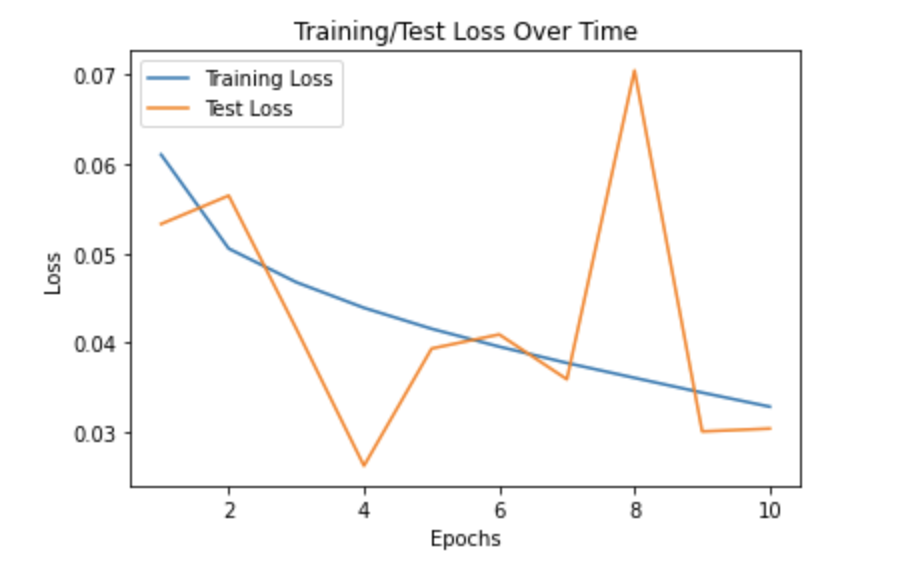
\includegraphics[width=.7\textwidth]{losses.png}

\item 
Model Train accuracy: 67 \%

Model Test accuracy: 54 \%

Model train precision for class 0 through 9, respectively: [0.70503876 0.81568228 0.53122172 0.60341151 0.60975104 0.54714384
 0.69519833 0.6999824  0.78943073 0.75186056]
 
Model train recall for class 0 through 9, respectively: [0.7276 0.801  0.587  0.3396 0.5878 0.636  0.7326 0.7956 0.7738 0.7678]

Model test precision for class 0 through 9, respectively: [0.62154433 0.68831169 0.43470149 0.38979964 0.46865365 0.43500425
 0.58760891 0.55611814 0.65875371 0.58519961]
 
Model test recall for class 0 through 9, respectively: [0.652 0.636 0.466 0.214 0.456 0.512 0.607 0.659 0.666 0.601]

Training Confusion Matrix:

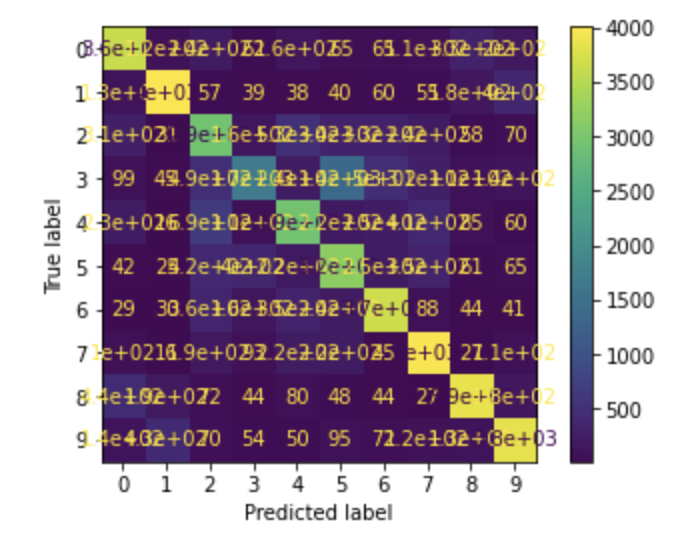
\includegraphics[width=.7\textwidth]{trainconfusion.png}

Test Confusion Matrix:

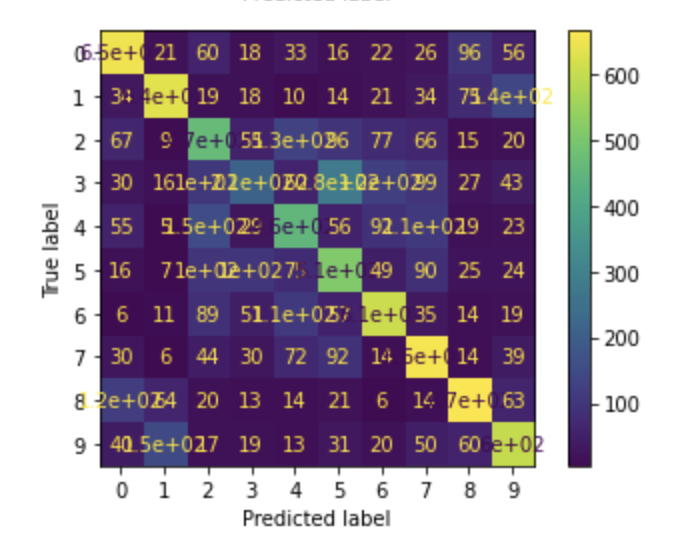
\includegraphics[width=.7\textwidth]{testconfusion.png}

Confusion matrices give us complete information on what is getting misclassifed as what (anything not on the diagonal are misclassified instances). Referencing the CIFAR-10 labels, we see that in training, we get a high proportion of cat images (label 3) getting a predicted label of dog (label 5). This intuitively makes sense since the two images might share many similarities. I was surprised that not many trucks (label 9) in training got mislabelled as cars (label 1). However, in test, we see that this misclassification is much more likely (as well as the opposite misclassification error). It also seems that the errors made in training and magnified (bright cells in the same places are even brighter in test). This might point to a need for more data, especially to be able to separate classes which might share similarities. For example, it seems that animals are hard for the model to distinguish between. 
\item For my new NN class, I know that generally bigger networks tend to be more predictive (more computational power = better classification), so I wanted to double the number of FC layers and double the number of nodes in each layer to see if this helps with classification:

\begin{lstlisting}
class Part2NeuralNetwork(nn.Module):
    def __init__(self):
        super(Part2NeuralNetwork, self).__init__()
        self.fc1 = torch.nn.Linear(3072, 2000) 
        self.fc2 = torch.nn.Linear(2000, 2000) 
        self.fc3 = torch.nn.Linear(2000, 2000) 
        self.fc4 = torch.nn.Linear(2000, 2000) 
        self.fc5 = torch.nn.Linear(2000, 2000) 
        self.fc6 = torch.nn.Linear(2000, 10) 

    def forward(self, x):
        self.batch_size = x.shape[0]
        x = x.view(self.batch_size, -1)
        x = F.relu(self.fc1(x))
        x = F.relu(self.fc2(x))
        x = F.relu(self.fc3(x))
        x = F.relu(self.fc4(x))
        x = F.relu(self.fc5(x))
        x = F.relu(self.fc6(x))
        return x
\end{lstlisting}

New NN Architecture Losses:

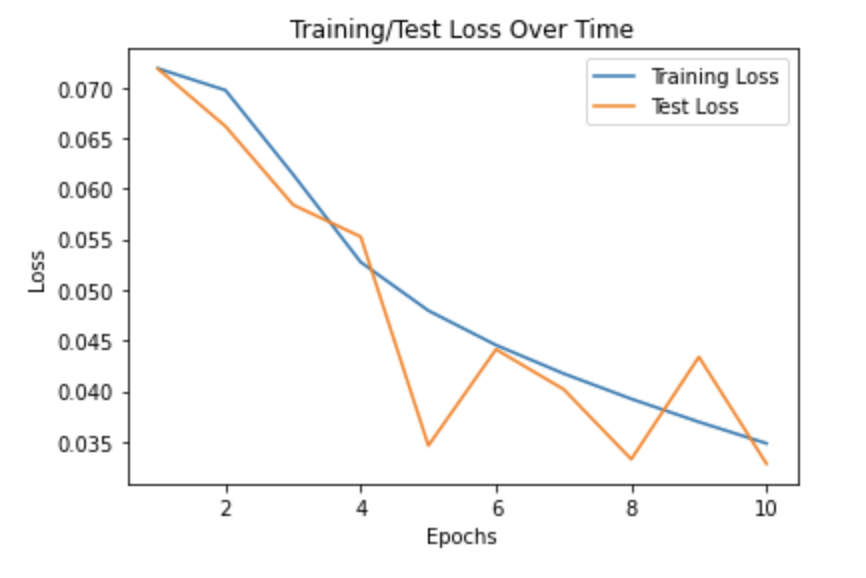
\includegraphics[width=.7\textwidth]{newlosses.png}

Model train accuracy: 64 \%

Model test accuracy: 53 \%

Model train precision for class 0 through 9, respectively: [0.69671653 0.76795367 0.59251031 0.42045099 0.54684299 0.51610954
 0.61956354 0.82261072 0.75475285 0.8591029 ]
 
Model train recall for class 0 through 9, respectively: [0.7172 0.7956 0.3734 0.537  0.5872 0.5126 0.8006 0.7058 0.794  0.6512]

Model test precision for class 0 through 9, respectively: [0.60309777 0.67255717 0.49917628 0.33111111 0.45352113 0.42745098
 0.52187029 0.67105263 0.63619744 0.68882603]
 
Model test recall for class 0 through 9, respectively: [0.623 0.647 0.303 0.447 0.483 0.436 0.692 0.561 0.696 0.487]

Model Train Confusion Matrix:

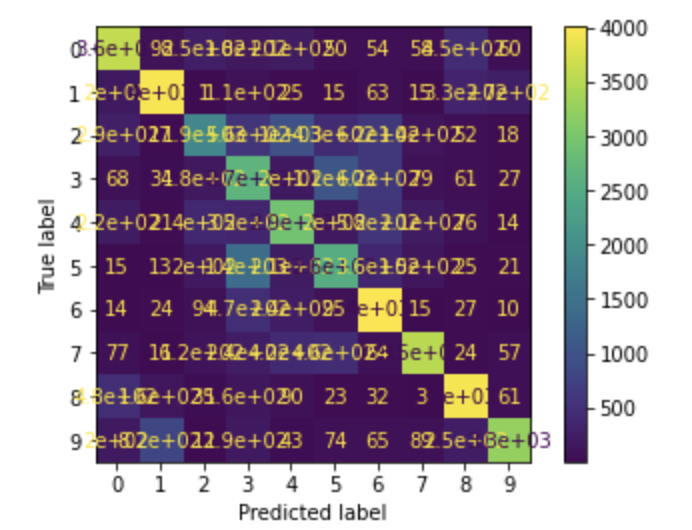
\includegraphics[width=.7\textwidth]{newtrainconfusion.png}

Model Test Confusion Matrix:

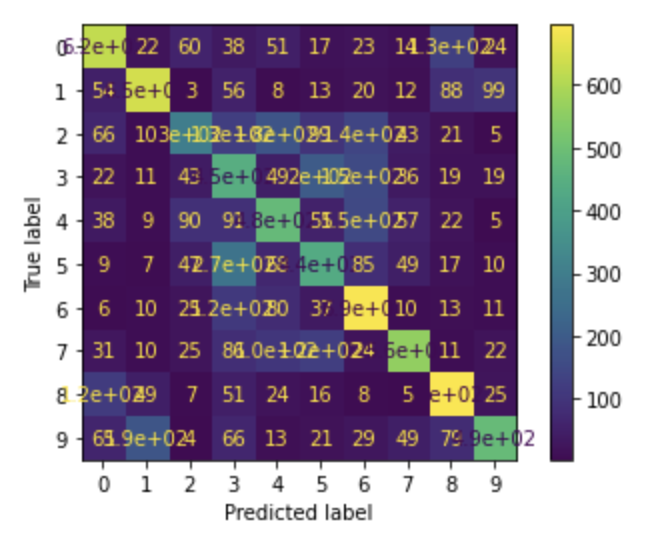
\includegraphics[width=.7\textwidth]{newtestconfusion.png}

From these confusion matrices, it seems that the issues cited for the original NN are exacerbated by this larger network. Things like cats and dogs, animals in general, and trucks vs. cars, are even harder for the model to distinguish. It might be possible that with a larger network, we need to train for longer to get the same results, but there are also other reasons this network performed worse (I tried a few runs, but it seemed consistently worse.) Perhaps, having fewer FC nodes means fewer features get passed between layers, and that the more pruned features are more characteristic, whereas with more layers and nodes, more noisy, non-predictive information gets passed between layers and impacts classification. Metrics for precision and recall are also worse, supporting the idea that for this particular classification task, a smaller FC network performs better. Perhaps there is also a ceiling on performance of FC networks for images, and a CNN would yield better results. 

\end{enumerate}
\newpage
%%%%%%%%%%%%%%%%%%%%%%%%%%%%%%%%%%%%%%%%%%%%%
% Name and Calibration
%%%%%%%%%%%%%%%%%%%%%%%%%%%%%%%%%%%%%%%%%%%%%
\subsection*{Name}

Kathryn Wantlin

\subsection*{Collaborators and Resources}
Whom did you work with, and did you use any resources beyond cs181-textbook and your notes?

Justine Boudou

Office Hours: Nari, Yash, Mark, Sanjana, Richard

Paper linked in Question 1.

\subsection*{Calibration}
Approximately how long did this homework take you to complete (in hours)? 

15 hrs.

\end{document}
